\documentclass[11pt]{beamer}

\usepackage[utf8]{inputenc} 
\usepackage[T1]{fontenc}
\usepackage{lmodern}
\usepackage{graphicx}
\usepackage[french]{babel}
\setbeamertemplate{blocks}[rounded][shadow=true]

% \onehalfspacing

% Espacement des lignes
\linespread{1.3}

% Theme
\usepackage{animate}
\usetheme{Frankfurt}                                % un theme voir .../beamer/theme/


% Numéro diapo en bas
\setbeamertemplate{footline}[frame number]

\title[segment SOL]{Projet DRONE}
\subtitle{Création de L'OS embarqué}
\institute{ Ecole Supérieure des Technologies Electronique Informatique Infographie  }
\author{Pierre-jean \textsc{TEXIER}}
\date{14 Février 2014}
 

 


\hypersetup{% Modifiez la valeur des champs suivants
	pdfauthor   = {auteur},%
	pdftitle    = {Titre},%
	pdfsubject  = {Sujet},%
	pdfkeywords = {Mots clés},%
	pdfcreator  = {PDFLaTeX},%
	pdfproducer = {PDFLaTeX},%
	pdfpagemode = {FullScreen}%                           % ouvre le pdf directement en plein écran
}


\begin{document}
	% Diapositive
	\begin{frame}
		\maketitle

		\begin{figure}
			\begin{center}
				
\includegraphics{commons/estei.png}
			\end{center}
		\end{figure}
		\begin{figure}
			\begin{center}
				
\includegraphics[width=1cm]{commons/cc.png}
			\end{center}
		\end{figure}
		
	\end{frame}
		
% 	\section{Sommaire}
%	\subsection{} ...
%   \subsubsection{} ...
	\begin{frame}
		\frametitle{Sommaire}
		%\framesubtitle{}
		\begin{columns}[t]
		\begin{column}{5cm}
		\tableofcontents[sections={1-4}]
		\end{column}
		\begin{column}{5cm}
		\tableofcontents[sections={5-8}]
		\end{column}
		\end{columns}
	 \end{frame}
	
 	\section{Introduction}
	\begin{frame}{Introduction}
		\begin{itemize}
			\item Segment SOL
		\end{itemize}
	\end{frame}

 	\section{Objectif}
	\begin{frame}
		\frametitle{Objectif}
		\framesubtitle{}
	\begin{block}{Tâches à réaliser}
		\begin{itemize}
			\item OS Linux embarqué Fonctionnel
			\item Préparation de l'environnement graphique (Qt, openCV, ...)
			\item Optimisation du temps de boot hardware et subjectif
			\item Gestion de l'énergie
		\end{itemize}
	\end{block}
	\end{frame}
	
	%%%%%%%%%%%%%%%%%%%%%%%%%%%%%%%%%%%%%%ù
	\section{Gestion de Projet}
	\subsection{Diagramme de GANTT}
	\begin{frame}{Gantt}
		\begin{center}
			Dans les jalons le long du projet\\
			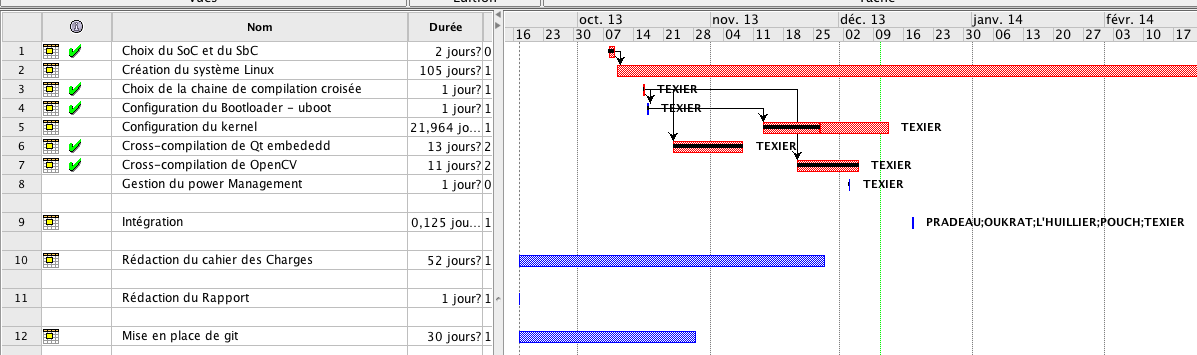
\includegraphics[width=10cm]{commons/Gantt.png}
		\end{center}
	\end{frame}
	
	\subsection{Diagramme PERT}
	\begin{frame}{Pert}
		\begin{center}
			
		\end{center}
	\end{frame}
	
	%%%%%%%%%%%%%%%%%%%%%%%%%%%%%%%%%%%%%%ù
	\section{Analyse Fonctionelle}
	\begin{frame}{Diagramme de séquence}
	
	\end{frame}
	
	%%%%%%%%%%%%%%%%%%%%%%%%%%%%%%%%%%%%%%ù
	\section{Réalisations}
	
	\begin{frame}{Réalisations}
		
		\begin{enumerate}
			\item<+-|alert@+> Choix technologiques
			\item<+-|alert@+> Environnement
			\item<+-|alert@+> U-boot
			\item<+-|alert@+> Kernel
			\item<+-|alert@+> RootFS
			\item<+-|alert@+> Qtembedded
			\item<+-|alert@+> OpenCV
			\item<+-|alert@+> Power Management
		\end{enumerate}
		
	\end{frame}
	
	\subsection{Choix technologiques}
	\begin{frame}{Choix technologiques}
	\begin{center}
		  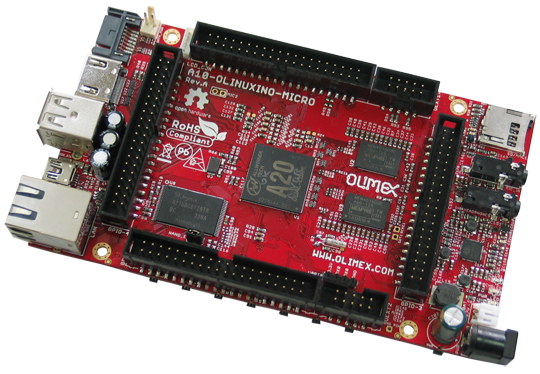
\includegraphics[width=4cm]{commons/A20-OLinuXino-MICRO-0.jpg}
		 \begin{itemize}
			\item SbC
			\item SoC
		\end{itemize}
	\end{center}
	\end{frame}
	
	\subsection{Environnement}
	\begin{frame}{Environnement}
	\begin{center}
	  
\includegraphics[width=2cm]{commons/linaro.jpeg}
	\end{center}
	\begin{itemize}
			\item gcc-linaro-arm-linux-gnueabihf-4.7-linux
			
\includegraphics[width=1cm]{commons/gnu.jpeg}
	\end{itemize}
	\begin{block}{Pourquoi armhf ?}
		FPU neon-vfvp4
	\end{block}
	\begin{block}{Pourquoi Linaro ?}
	\begin{itemize}
	      \item CodeSourcery
	      \item Crosstool-ng
	      \item Buildroot
	\end{itemize}
	\end{block}
	\end{frame}
	
	\subsection{U-boot}
	\begin{frame}{U-boot}
		\begin{block}{Informations}
		\begin{itemize}
			\item Non mainline - Git du projet sunxi
			\href{https://github.com/linux-sunxi/u-boot-sunxi}{\beamergotobutton{Lien github}}
		\end{itemize}
	\end{block}
	Configuration en statique dans : /include/configs/sunxi-common.h
	\end{frame}
	
	\subsection{Kernel}
	\begin{frame}{Kernel}
	
\includegraphics[width=1cm]{commons/tux.png}
		\begin{block}{Informations}
		\begin{itemize}
			\item Version 3.4.67
			\item Non mainline - Git du projet sunxi
			\href{https://github.com/linux-sunxi/linux-sunxi}{\beamergotobutton{Lien github}}
		\end{itemize}
	\end{block}
	\end{frame}
	
	\subsection{RootFS}
	\begin{frame}{RootFS}
		\begin{center}
			
		\end{center}
	\end{frame}
	
	\subsection{Qt embedded}
	\begin{frame}{Qt embedded}
		\begin{center}
			  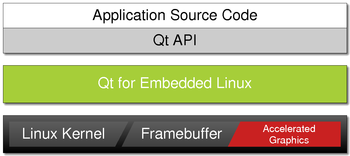
\includegraphics[width=4cm]{commons/qt-embedded-linux-architecture.png}
		\end{center}
			  Portage sur cible Arm Cortex A7 : 
		\begin{itemize}
			  \item<+-|alert@+> Qt embedded 4.8.2
			  \item<+-|alert@+> Librairie touchscreen tslib
			  \item<+-|alert@+> Divers exemples Qt4
		\end{itemize}
	\end{frame}
	
	\subsection{OpenCV embedded}
	\begin{frame}{OpenCV embedded}
		\begin{center}
			
		\end{center}
	\end{frame}
	
	\subsection{Power Management}
	\begin{frame}{Power Management}
		\begin{columns}[t]
		\begin{column}{5cm}
		AXP209
		\end{column}
		\begin{column}{5cm}
		AXP209
		\end{column}
		\end{columns}
		
	\end{frame}
	
	%%%%%%%%%%%%%%%%%%%%%%%%%%%%%%%%%%%%%%ù
	\section{Conclusion}
	\begin{frame}{Conclusion}
		\begin{center}
		\begin{itemize}
			\item Apport ...
		\end{itemize}
		\end{center}
	\end{frame}
\end{document}
